\documentclass[12pt, a4paper]{article}
\usepackage[margin=1in]{geometry}
\usepackage{graphicx}
\usepackage{float}
\usepackage{booktabs}
\usepackage{hyperref}
\setlength{\parindent}{0pt}
\setlength{\parskip}{0.5pt}

\title{
    \vspace{-1cm}
    \Large\textbf{Bike Sharing Demand Forecasting:\\}
}
\author{
    William Chen
}
\date{}

\begin{document}
\maketitle
\thispagestyle{empty}

%-----------------------------------------------------------------------
\begin{abstract}
This report analyses daily bike rental counts from the UCI Bike Sharing
Dataset, comprising 731 observations collected from the Capital Bikeshare
system in Washington D.C.\ between 2011 and 2012. Since \textit{cnt} is
a non-negative integer, Poisson GLM is a more theoretically appropriate
choice than OLS. However, the raw Variance/Mean ratio of 833 and a
post-fit dispersion estimate of 182.6 reveal severe overdispersion,
violating the Poisson assumption of equal mean and variance. Negative
Binomial regression (NB2) is adopted to address this, reducing the
dispersion estimate to 1.046 and the AIC from 137,807 to 12,193.
Zero-Inflated Poisson (ZIP) is found inapplicable as the minimum observed
count is 22. The final NB2 model achieves a McFadden $R^2$ of 0.761 and identifies \textit{temp} (IRR $= 4.51$), \textit{yr1} (IRR $= 1.62$),
and \textit{weathersit3} (IRR $= 0.48$) as the dominant predictors of
daily rental demand.
\end{abstract}

\newpage
%-----------------------------------------------------------------------
\section{Introduction}
Bike-sharing systems have become an increasingly popular form of urban
transportation, offering a flexible and environmentally friendly
alternative to private vehicles. Accurately forecasting daily rental
demand is valuable for operators seeking to optimise fleet distribution,
staffing, and infrastructure planning. Demand is inherently influenced
by a combination of weather conditions, seasonal patterns, and calendar
effects, making it a well-suited problem for regression modelling.

This report analyses daily bike rental counts using the UCI Bike Sharing
Dataset, which records 731 days of rental activity across 2011 and 2012
in Washington D.C. Since the response variable \textit{cnt} is a
non-negative integer, count regression is more theoretically appropriate
than Ordinary Least Squares. We begin with Poisson GLM as the canonical
model for count data, and address the overdispersion present in the data
using Negative Binomial regression (NB2). Zero-Inflated Poisson (ZIP) is
also considered but found inapplicable given the absence of zero counts
in the dataset. Model performance is evaluated using AIC, BIC, dispersion
estimate, and McFadden $R^2$, with coefficients interpreted via Incidence
Rate Ratios (IRR $= e^{\hat{\beta}}$).

%-----------------------------------------------------------------------
\section{Data}

\subsection{Dataset Overview}
The dataset contains 731 daily observations collected between January 2011 and
December 2012 from the Capital Bikeshare system. It comprises 16 variables,
including temporal indicators, weather measurements, and rental usage counts.
No missing values were found. The target variable \textit{cnt} represents the
total number of bike rentals per day, combining both casual and registered users.

\subsection{Feature Description}
The dataset contains 16 variables: 2 identifiers (\textit{instant}, \textit{dteday},
excluded from analysis), 1 continuous target (\textit{cnt}), and 13 predictors.
Features span temporal (\textit{season}, \textit{yr}, \textit{mnth}, \textit{holiday},
\textit{weekday}, \textit{workingday}), weather (\textit{weathersit}, \textit{temp},
\textit{atemp}, \textit{hum}, \textit{windspeed}), and usage (\textit{casual},
\textit{registered}) dimensions. Among the 13 predictors, 7 are categorical and
4 are continuous.

\subsection{Feature Selection and Preprocessing}
Prior to modelling, four variables were removed from the dataset.
\textit{instant} and \textit{dteday} are excluded as they serve purely as
a record index and a date string respectively, carrying no predictive
information. \textit{casual} and \textit{registered} are excluded due to
target leakage: they are direct components of \textit{cnt} (i.e.\
$\textit{cnt} = \textit{casual} + \textit{registered}$), and including them
would trivially inflate model performance without providing genuine
predictive value. Further variables (\textit{atemp}, \textit{mnth},
\textit{workingday}) are examined and removed in subsequent sections based
on correlation analysis and multicollinearity diagnostics.

%-----------------------------------------------------------------------
\section{Exploratory Data Analysis}

\subsection{Feature Distribution}

Figure~\ref{fig:cnt_dist} shows the distribution of daily rental counts.
Counts range from 22 to approximately 8,700. The distribution is
roughly symmetric but exhibits a slight secondary peak around 7,000--7,500,
likely reflecting the higher overall demand in 2012 compared to 2011.

\begin{figure}[H]
    \centering
    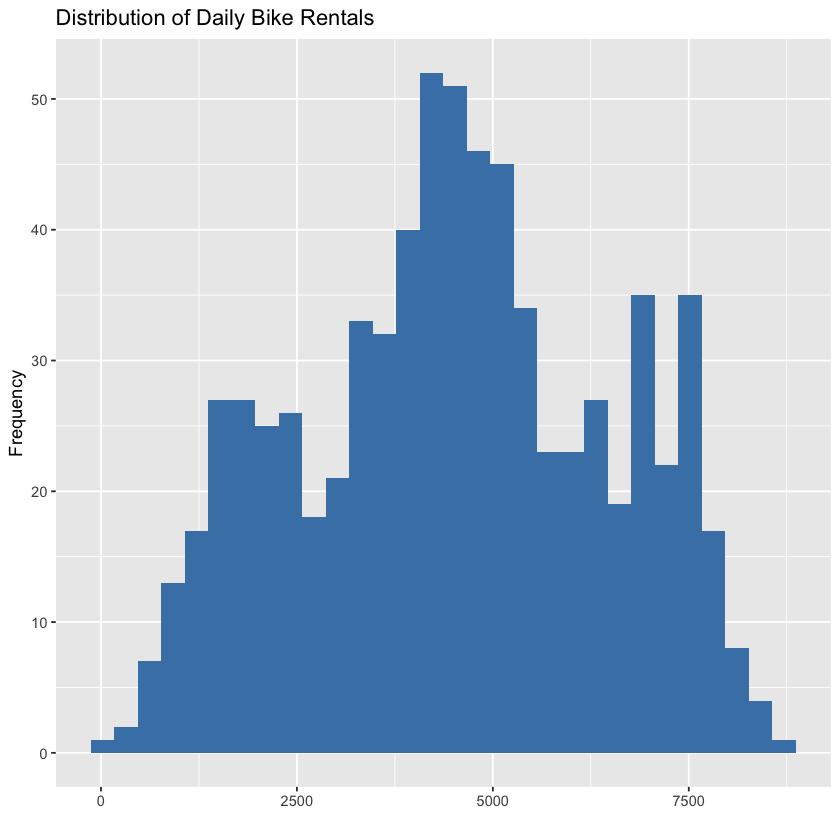
\includegraphics[width=0.7\textwidth]{figures/cnt_histogram.png}
    \caption{Distribution of Daily Bike Rentals}
    \label{fig:cnt_dist}
\end{figure}
 
\subsubsection{Categorical Features}

Figures~\ref{fig:boxplot_season} and~\ref{fig:boxplot_month} show
consistent seasonal trends: counts peak in Summer, followed by Spring
and Fall, while Winter records the lowest demand. The two plots convey
near-identical distributional patterns, reflecting the strong overlap
between the two variables.

Figure~\ref{fig:boxplot_yr} shows a marked increase in overall demand from
2011 (Year 0) to 2012 (Year 1), with the median rising from approximately
3,500 to 6,200. A small number of outliers are visible across all three
plots, representing isolated days with unusually low counts; these are
consistent with extreme weather events and are considered a normal
occurrence in the data.


\begin{figure}[H]
    \centering
    \begin{minipage}{0.48\textwidth}
        \centering
        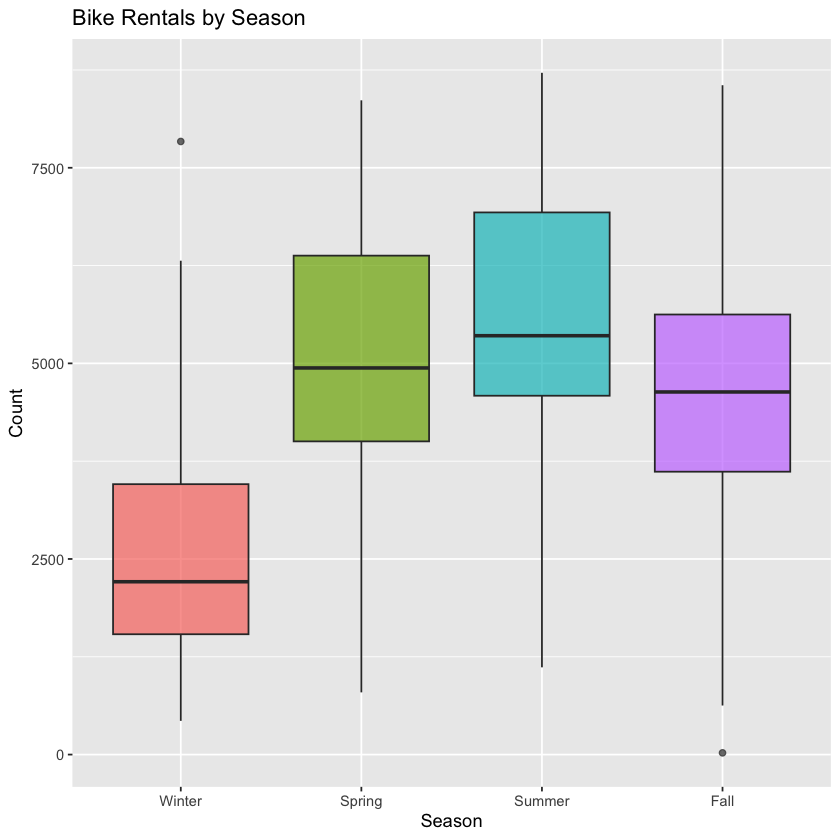
\includegraphics[width=\textwidth]{figures/season_boxplot.png}
        \caption{Bike Rentals by Season}
        \label{fig:boxplot_season}
    \end{minipage}
    \hfill
    \begin{minipage}{0.48\textwidth}
        \centering
        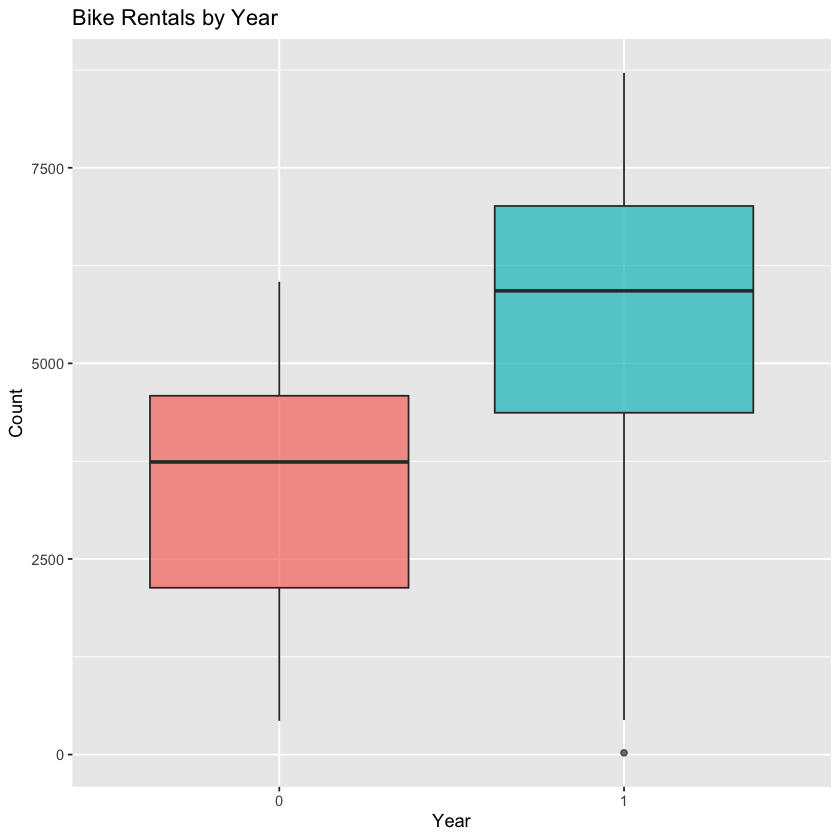
\includegraphics[width=\textwidth]{figures/year_boxplot.png}
        \caption{Bike Rentals by Year}
        \label{fig:boxplot_yr}
    \end{minipage}
\end{figure}
 
\begin{figure}[H]
    \centering
    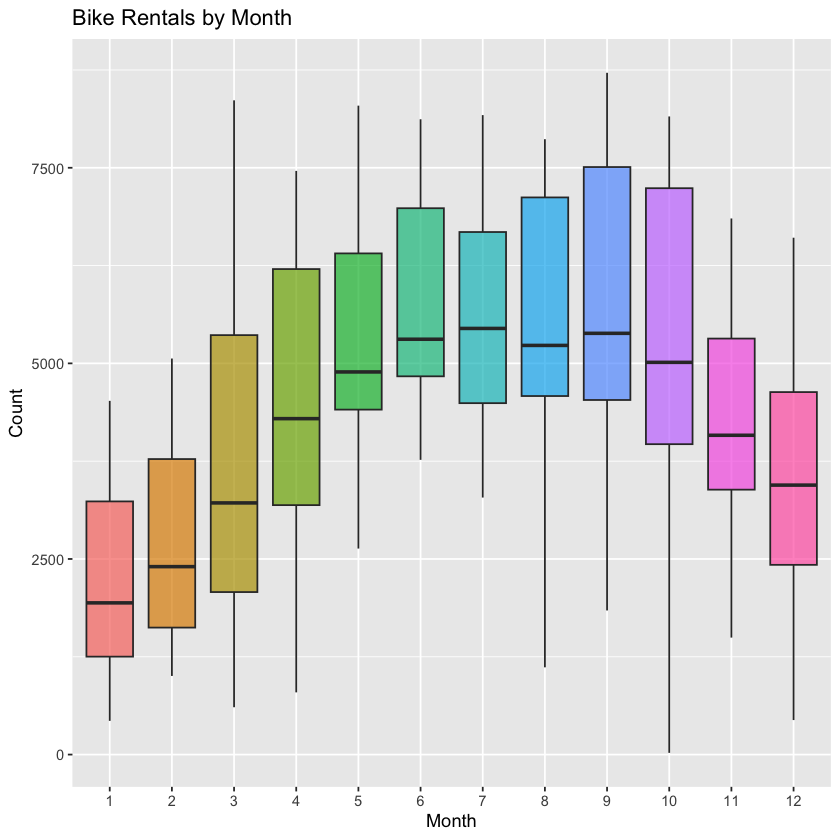
\includegraphics[width=0.6\textwidth]{figures/month_boxplot.png}
    \caption{Bike Rentals by Month}
    \label{fig:boxplot_month}
\end{figure}

Figure~\ref{fig:boxplot_weather} shows rental counts across weather
conditions and day-type indicators. \textit{weathersit} shows a clear
negative trend: higher values indicate more severe weather, and rental
counts decline accordingly. Level 4 does not appear in the dataset as no
such extreme weather days were recorded. \textit{holiday},
\textit{weekday}, and \textit{workingday} show largely overlapping
distributions with no strong separation between categories.

\begin{figure}[H]
    \centering
    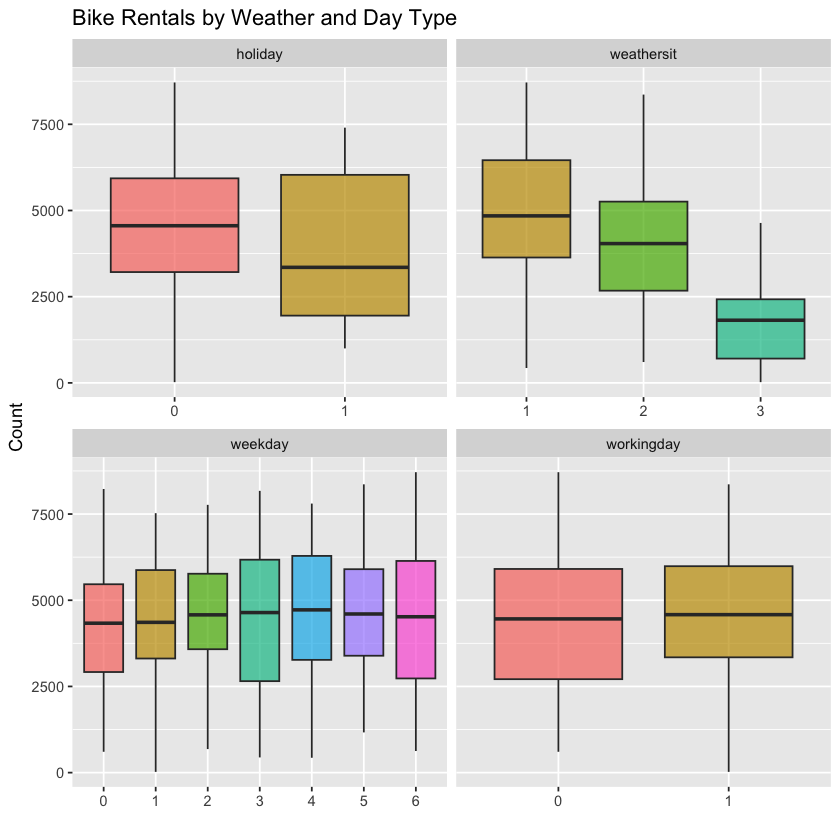
\includegraphics[width=0.55\textwidth]{figures/weather_daytype_boxplot.png}
    \caption{Bike Rentals by Weather and Day Type}
    \label{fig:boxplot_weather}
\end{figure}
 
\subsubsection{Numeric Features}

Figure~\ref{fig:scatter_numeric} shows the relationship between each
numeric feature and daily rental counts. Both \textit{temp} and
\textit{atemp} display near-identical positive trends, suggesting that
the two variables carry largely redundant information. \textit{hum} and
\textit{windspeed} both show negative relationships with rental counts,
indicating that higher humidity and stronger winds are associated with
fewer rentals.

\begin{figure}[H]
    \centering
    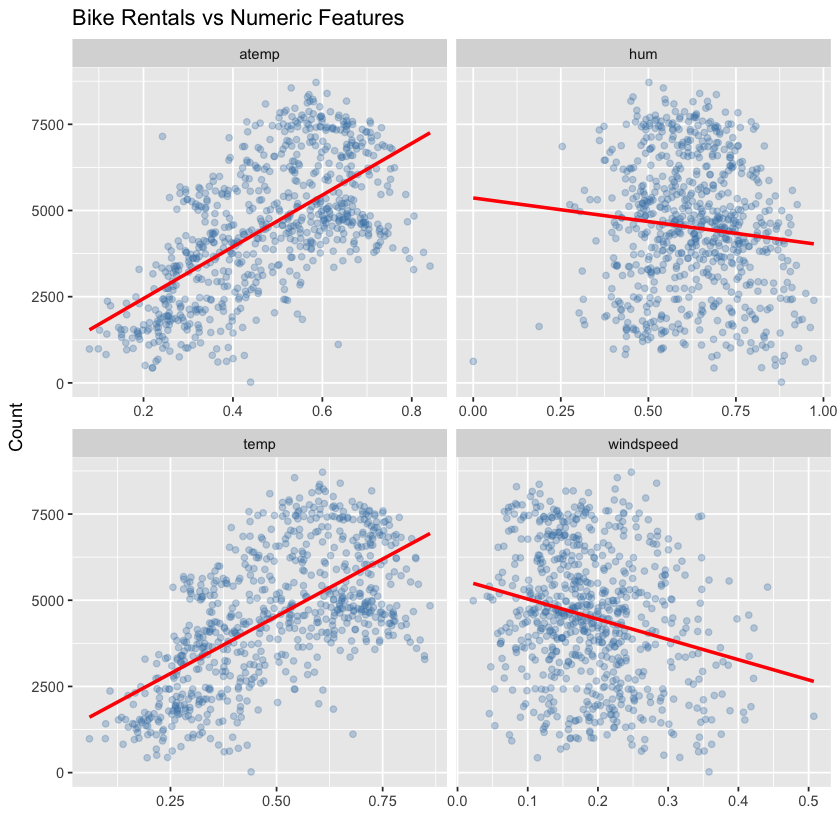
\includegraphics[width=0.55\textwidth]{figures/numeric_scatter.png}
    \caption{Bike Rentals vs Numeric Features}
    \label{fig:scatter_numeric}
\end{figure}

\subsection{Feature Correlation}

Figure~\ref{fig:corr_matrix} shows the correlation matrix for numeric
features. The most notable finding is the near-perfect correlation between
\textit{temp} and \textit{atemp} ($r = 0.99$), confirming the visual
observation from the scatter plots and providing a clear justification for
removing one of the two variables. Both \textit{hum} ($r = -0.10$) and
\textit{windspeed} ($r = -0.23$) show negative correlations with
\textit{cnt}, consistent with the trends observed earlier.

\begin{figure}[H]
    \centering
    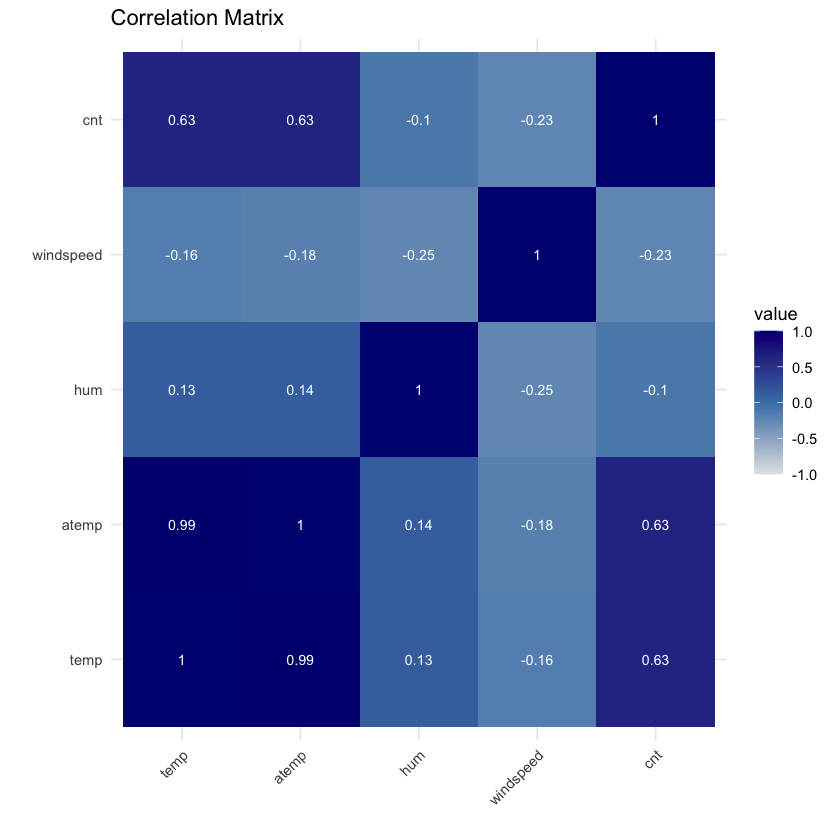
\includegraphics[width=0.7\textwidth]{figures/correlation_matrix.png}
    \caption{Correlation Matrix of Numeric Features}
    \label{fig:corr_matrix}
\end{figure}

\subsection{Multicollinearity Check (VIF)}
 
Variance Inflation Factor (VIF) was computed to assess multicollinearity
among the remaining predictors. Before running VIF, three variables were
excluded from the model: \textit{atemp} (near-perfect correlation with
\textit{temp}, $r = 0.99$), \textit{mnth} (aliased with \textit{season}),
and \textit{workingday} (linearly derived from \textit{weekday} and
\textit{holiday}). Including aliased variables causes perfect
multicollinearity, making VIF computation impossible due to a singular
design matrix.
 
All remaining features returned VIF values below 3.6, indicating no
problematic multicollinearity. The two highest values belong to
\textit{season} (3.54) and \textit{temp} (3.41), which reflects a natural
association between temperature and season and does not warrant further
action.
 

%-----------------------------------------------------------------------
%-----------------------------------------------------------------------
\section{Methodology}

\subsection{Poisson GLM}

Poisson GLM is a generalised linear model suited for count data. It uses a
log link function to model the expected count, ensuring all predicted values
remain non-negative. The key advantage over OLS is that it respects the
discrete, non-negative nature of the response variable. Coefficients are
interpreted through the Incidence Rate Ratio (IRR = $e^\beta$), which
represents the multiplicative change in expected count for a one-unit
increase in a predictor. A core assumption of Poisson is equidispersion,
meaning the variance equals the mean. Violation of this assumption leads to
underestimated standard errors and unreliable inference.

\subsection{Negative Binomial (NB2)}

Negative Binomial regression is an extension of Poisson that introduces an
additional dispersion parameter, allowing the variance to exceed the mean.
It is the standard approach when overdispersion is detected in count data.
Coefficients are interpreted in the same way as Poisson via IRR. When the
dispersion parameter is very large, NB2 converges to Poisson, making
Poisson a special case of NB2.

\subsection{Zero-Inflated Poisson (ZIP)}

ZIP is designed for count data with an excess of zero observations. It
models zeros as arising from two sources: a structural zero component and
a count component. ZIP is considered when the number of zeros in the data
exceeds what Poisson or NB2 would predict. In this dataset, the minimum
observed count is 22 with no zero counts present, so ZIP is not applicable
and is excluded from further analysis.

\subsection{Evaluation Metrics}

Models are compared using AIC and BIC, which balance goodness of fit
against model complexity. Lower values indicate a better model. The
dispersion estimate (Residual Deviance / degrees of freedom) is used to
verify whether the equidispersion assumption holds, with values close to 1
indicating a well-fitted model. McFadden $R^2$ serves as a supplementary
goodness-of-fit measure; however, it should be interpreted with caution
under Poisson when overdispersion is present, as the inflated deviance can
produce artificially high values. Binned residual plots provide a visual
check of model fit by examining whether average residuals fall within the
95\% confidence bands.

\paragraph{Quasi-Poisson.}
An alternative approach for handling overdispersion is Quasi-Poisson, which
corrects standard errors by scaling them with the dispersion estimate without
changing the coefficients. However, since Quasi-Poisson does not produce a
full likelihood, AIC and BIC cannot be computed, making formal model
comparison infeasible. Negative Binomial regression is therefore preferred
in this analysis.

%-----------------------------------------------------------------------
\section{Results}

\subsection{Poisson GLM}

A preliminary dispersion check on the raw data reveals a Variance/Mean ratio
of 833.15, indicating severe overdispersion before any model is fitted.
After fitting the Poisson GLM, the post-fit dispersion estimate (Residual
Deviance / df) drops to 182.6, which still far exceeds 1, confirming that
the Poisson assumption of equidispersion is violated even after controlling
for all predictors.

Figure~\ref{fig:binned_poisson} shows the binned residual plot for the
Poisson model. The majority of points fall outside the 95\% confidence
bands (grey lines), with residuals ranging from approximately $-18$ to $9$.
This visually confirms the poor fit of the Poisson model and motivates the
use of Negative Binomial regression.

\begin{figure}[H]
    \centering
    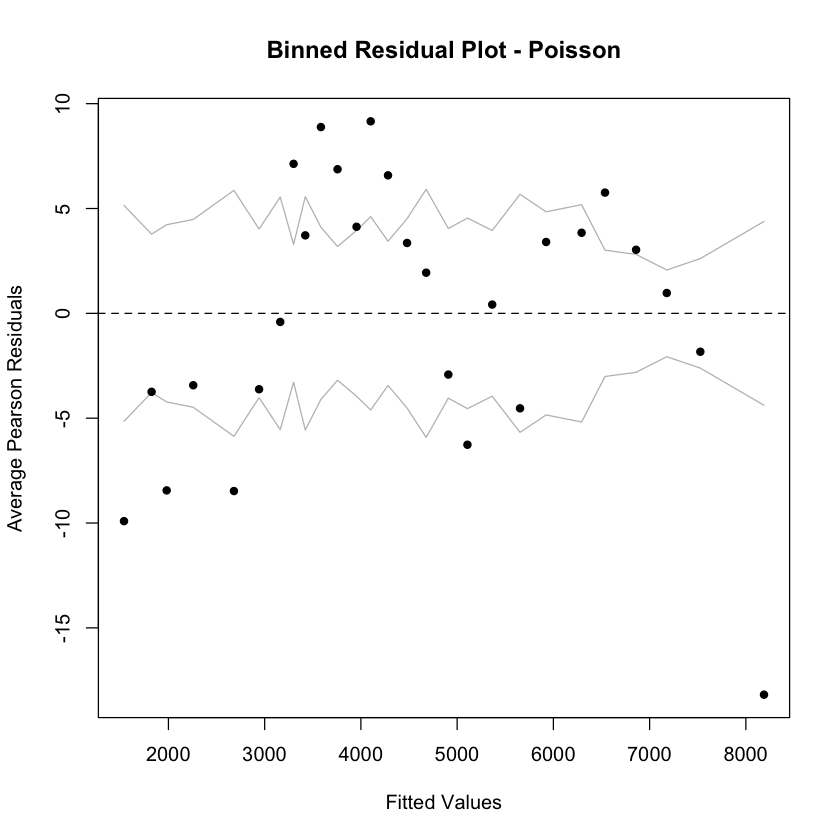
\includegraphics[width=0.6\textwidth]{figures/binned_residual_poisson}
    \caption{Binned Residual Plot --- Poisson GLM}
    \label{fig:binned_poisson}
\end{figure}


\subsection{Negative Binomial (NB2)}

The NB2 model yields a dispersion estimate of 1.046 (Residual Deviance
747.07 / df 714), a substantial improvement from the Poisson model's
182.6, indicating that the overdispersion is successfully resolved.

Figure~\ref{fig:binned_nb2} shows the binned residual plot for NB2.
Compared to Poisson, the y-axis range narrows dramatically from
approximately $[-18, 9]$ to $[-1.0, 0.75]$, and the majority of points
fall within the 95\% confidence bands. A small number of points near the
lower and upper ends of the fitted value range fall slightly outside,
suggesting minor difficulties in predicting very low or very high demand
days.

\begin{figure}[H]
    \centering
    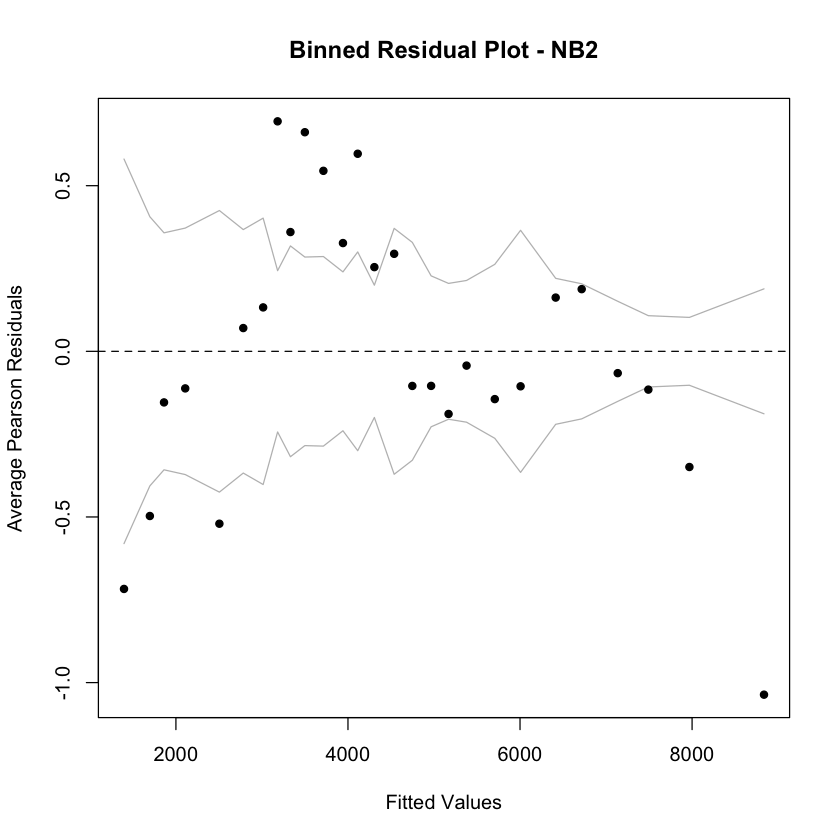
\includegraphics[width=0.6\textwidth]{figures/binned_residual_nb2}
    \caption{Binned Residual Plot --- NB2}
    \label{fig:binned_nb2}
\end{figure}

Figure~\ref{fig:actual_pred} shows the actual versus predicted counts.
Points align closely along the 45-degree reference line across the full
range of demand, confirming good overall predictive performance. Slight
deviations are observed at very low and very high counts, reflecting the
inherent difficulty of modelling extreme demand days.

\begin{figure}[H]
    \centering
    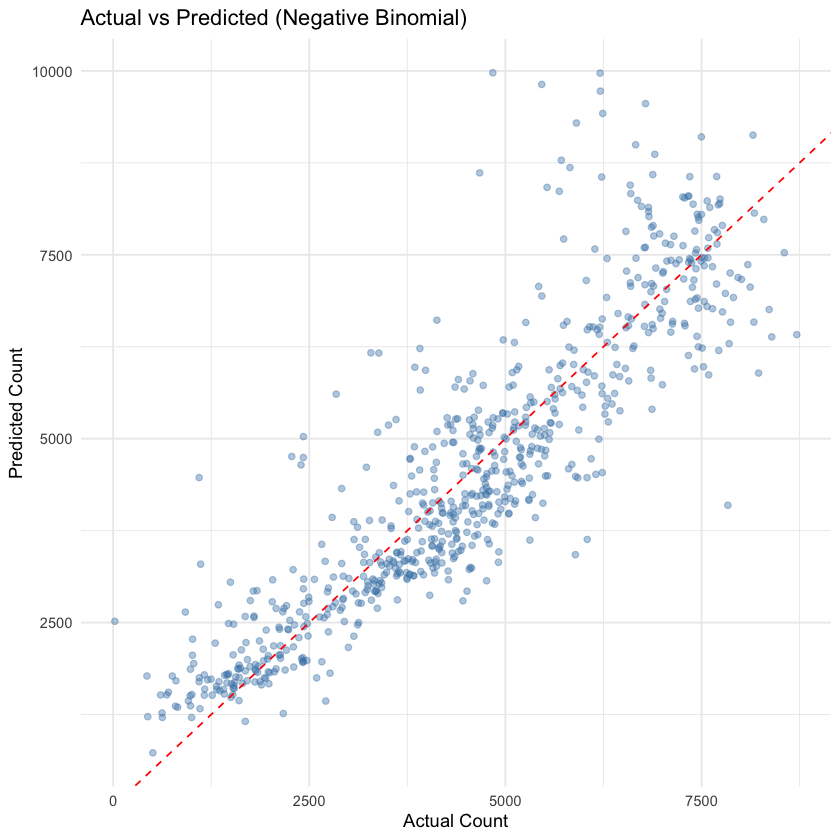
\includegraphics[width=0.6\textwidth]{figures/actual_vs_predicted_nb2}
    \caption{Actual vs Predicted --- NB2}
    \label{fig:actual_pred}
\end{figure}

The estimated coefficients, expressed as Incidence Rate Ratios, 
reveal the following key effects.
\textit{temp} has the largest positive effect
(IRR $= 4.508$, 95\% CI: $[3.755, 5.412]$), reflecting the strong
sensitivity of cycling demand to thermal comfort. \textit{yr1}
(IRR $= 1.619$, 95\% CI: $[1.561, 1.678]$) captures year-over-year
service growth from 2011 to 2012. \textit{seasonFall} shows the highest
seasonal effect (IRR $= 1.616$), with autumn demand approximately 62\%
higher than the Winter baseline.

On the negative side, \textit{weathersit3} (IRR $= 0.483$) indicates that
snow or rain days are associated with roughly half the demand of clear days,
and \textit{windspeed} (IRR $= 0.506$) similarly suppresses demand.
Among weekday indicators, \textit{weekday1} is the only non-significant
coefficient (95\% CI: $[0.996, 1.143]$ includes 1), suggesting that
Monday demand does not differ meaningfully from the Sunday baseline.



\subsection{Model Comparison}
Candidate models are compared using AIC, BIC, dispersion estimate, and
McFadden $R^2$. Lower AIC and BIC indicate better fit relative to model
complexity, while a dispersion estimate close to 1 confirms the
variance assumption is satisfied.

Table~\ref{tab:model_compare} summarises the two models across four metrics.

\begin{table}[H]
    \centering
    \caption{Model Comparison}
    \label{tab:model_compare}
    \begin{tabular}{lrrrr}
        \toprule
        \textbf{Model} & \textbf{AIC} & \textbf{BIC} & \textbf{Dispersion} & \textbf{McFadden $R^2$} \\
        \midrule
        Poisson & 137,806.50 & 137,884.61 & 182.596 & 0.805 \\
        NB2     &  12,193.16 &  12,275.86 &   1.046 & 0.761 \\
        \bottomrule
    \end{tabular}
\end{table}

NB2 outperforms Poisson across AIC and BIC by a large margin, and its
dispersion estimate of 1.046 confirms that overdispersion is resolved.
Although the Poisson model yields a higher McFadden $R^2$ (0.805 vs.\
0.761), this is an artifact of overdispersion inflating the deviance-based
statistic and should not be interpreted as evidence of better fit.
NB2 is therefore selected as the final model.


%-----------------------------------------------------------------------
\section{Discussion}

\subsection{Key Findings}

The NB2 model outperforms the Poisson GLM, as evidenced by lower AIC and
BIC and a dispersion estimate close to 1, indicating that the
equidispersion assumption is well-satisfied after accounting for the
overdispersion present in the raw data. Temperature (IRR $= 4.51$) is
the dominant predictor, with year-over-year growth (IRR $= 1.62$) and
seasonal effects also contributing substantially. Adverse weather and
high wind speed suppress demand by roughly half, while most weekday
effects are significant except Monday, which does not differ detectably
from the Sunday baseline.

\subsection{Limitations}

Three limitations are worth noting. First, the model covers only two
years of data, and the large \texttt{yr} coefficient may reflect a
growth phase specific to that period rather than a persistent trend,
limiting predictive validity for future years. Second, prediction errors
are likely larger on extreme weather days, as such events are rare and
poorly represented during training. Third, the model excludes interaction
terms such as \texttt{temp:season}, which may capture more nuanced
demand dynamics and improve performance.

\begin{thebibliography}{9}
 
\bibitem{fanaee2013}
Fanaee-T, H. (2013).
\textit{Bike Sharing} [Dataset].
UCI Machine Learning Repository.
\texttt{https://doi.org/10.24432/C5W894}
 
\end{thebibliography}

\end{document}